% 商拓扑
\pentry{二元关系\upref{Relat},映射\upref{map},拓扑空间\upref{Topol}}

\subsection{商集}

拓扑空间本身作为一个集合,可以在其上定义某种等价关系,由此可以得到等价类所构成的\textbf{商集}.我们可以将同一个等价类中的点看成是同一个点,把商集看成是原集合中部分点相互粘合所得到的集合.

\begin{example}{烟卷}\label{Topo7_ex1}
在$\mathbb{R}^2$中取一个矩形的闭子集:$A=\{(x,y)\in\mathbb{R}^2:x\in[-1,1],y\in[0,1]\}$.在这个闭子集上定义一个等价关系$\sim$如下:对于$y\in[0,1]$,有$(1, y)\sim(-1, y)$;其它点都只和自己等价.如果把$A$看成一个矩形纸条,那么商集$A/\sim$可以看成是这个纸条的两边对应点粘在一起,卷成一个烟卷的样子.

\begin{figure}[ht]
\centering
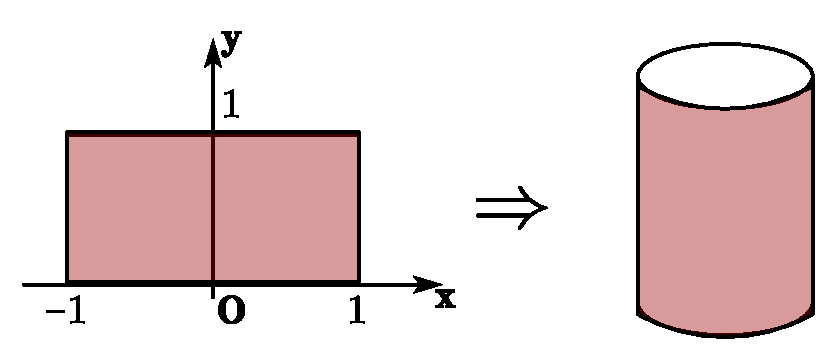
\includegraphics[width=8cm]{./figures/Topo7_1.pdf}
\caption{卷纸条的过程示意.左边是矩形纸条$A$,右边是模去等价关系$\sim$(或者说把等价的点粘在一起)以后得到的集合.} \label{Topo7_fig1}
\end{figure}

\end{example}



我们给出纸条$A$的准确坐标只是为了方便描述上述等价关系.实际上,在$\mathbb{R}^2$中选择任意的有界连通闭子集,都可以找到这个闭子集和$A$的同胚映射,在拓扑意义下它们就是相同的集合.取一个任意的四边形、三角形或者不规则图形都可以,你可以直观地想象成揉捏一个橡皮泥,只要不撕裂它,不把本来分开的点粘在一起,那揉出来的任何形状都是同胚的.当然,用矩形纸条描述以上商集最为方便.

\begin{example}{甜甜圈}

还是利用\autoref{Topo7_ex1}中的$A$,这次等价关系$\sim$为:对于$x\in[-1,1], y\in[0,1]$,有$(x,0)\sim(x,1), (1, y)\sim(-1, y)$,其它点只和自己等价.这一次,商集$A/\sim$可以看成把纸条的左右两边粘合,上下两边也粘合.先粘合哪些点并没有要求,所以可以先粘合成烟卷,再粘合成甜甜圈或者说轮胎的形状.

\end{example}

这种粘合若干边的商集很常见,我们可以定义一种图形化的表示方法,来表示等价关系.以烟卷为例,我们把待粘合的边表示为一个箭头,取名为$x$,然后把两个$x$箭头按照“头对头,尾对胃”的方向粘在一起,如图所示:

\begin{figure}[ht]
\centering
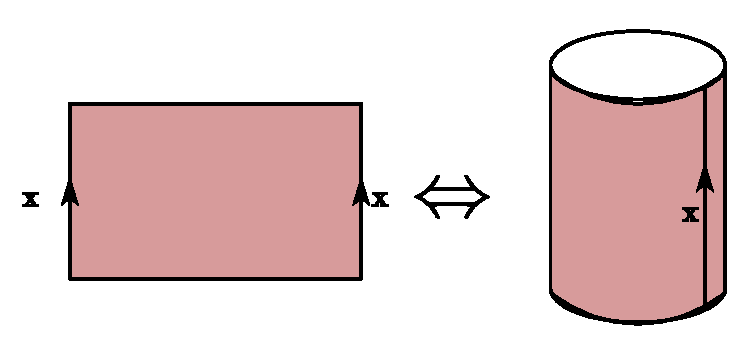
\includegraphics[width=8cm]{./figures/Topo7_2.pdf}
\caption{名称相同的箭头视为同一个,把它们粘连在一起.图示两个形状是相同的,左边的有两个同为$x$的箭头,要把它们粘连起来,结果是烟卷形状;右边只有一个箭头,不用进行粘连操作了,它本身也就是烟卷形状.} \label{Topo7_fig2}
\end{figure}

用这种箭头表示法,也可以通过在矩形上标注箭头$x$和$y$来表示一个甜甜圈:

\begin{figure}[ht]
\centering
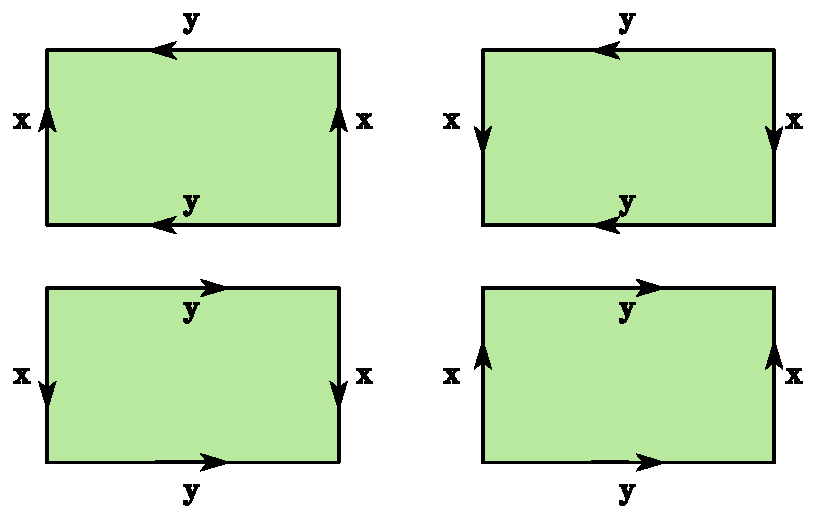
\includegraphics[width=8cm]{./figures/Topo7_3.pdf}
\caption{甜甜圈的四种箭头表示方法.这四种方法是完全等价的.} \label{Topo7_fig3}
\end{figure}

\begin{example}{莫比乌斯环}
用箭头表示法可以很轻松地表示一个\textbf{莫比乌斯环(Mobius)}.考虑到莫比乌斯环是把纸条的一边翻转以后再和对边粘连而成的,我们可以如\autoref{Topo7_fig4}画出莫比乌斯环的箭头表示法.如果只涉及一组边的粘合,我们可以在不引起混淆的情况下省去对箭头的命名.

\begin{figure}\label{Topo7_fig6}[ht]
\centering
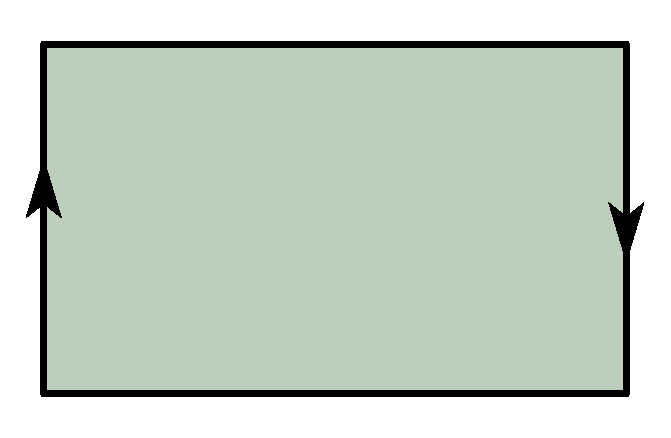
\includegraphics[width=5cm]{./figures/Topo7_4.pdf}
\caption{一个莫比乌斯环.将两个未命名的箭头粘在一起} \label{Topo7_fig4}
\end{figure}

\end{example}



\begin{example}{克莱因瓶}
用箭头表示法来表示一个\textbf{克莱因瓶(Klein's Bottle)}:
\begin{figure}[ht]
\centering
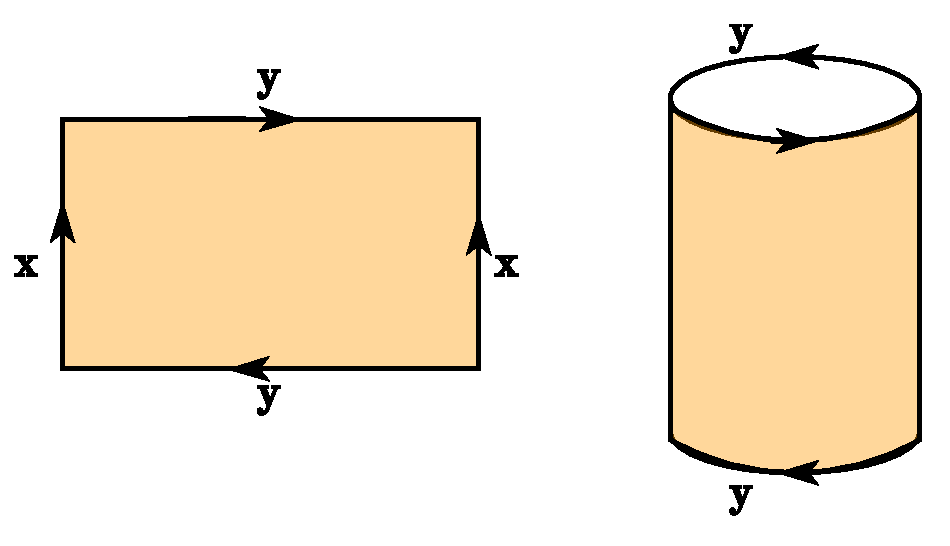
\includegraphics[width=8cm]{./figures/Topo7_5.pdf}
\caption{克莱因瓶的一种表示.我们可以把克莱因瓶看成先把$x$粘起来,再把$y$粘起来的操作,同样也可以看成先粘连$y$再粘连$x$,只是后一种思路复杂得多,更难想象.} \label{Topo7_fig5}
\end{figure}

注意克莱因瓶的定义中,两个$y$箭头的朝向相反.如果先粘连$y$箭头的话,所得到的就是一个莫比乌斯环,由此可以看出莫比乌斯环和克莱因瓶的相似性.

\end{example}

\begin{example}{射影平面}

射影平面和克莱因瓶、莫比乌斯带一样,如果一只蚂蚁在射影平面上爬行并且不离开平面也不触及边缘,它总能爬到出发点的对面.用箭头表示法来表示摄影平面如下:

\begin{figure}[ht]
\centering
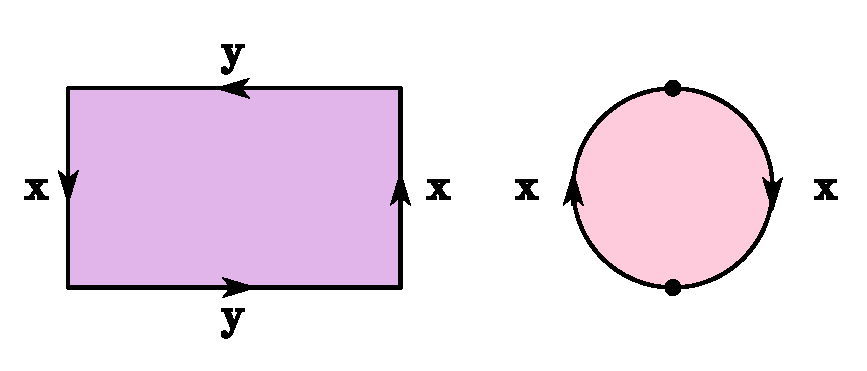
\includegraphics[width=8cm]{./figures/Topo7_8.pdf}
\caption{射影平面示意图.矩形和圆形的示意图是等价的.射影平面很难直观地画出来,多数情况下只能这样表示.} \label{Topo7_fig8}
\end{figure}

如果在射影平面的中间挖去一个洞,那么我们就得到了莫比乌斯带.射影平面实际上是莫比乌斯带将边缘粘连起来的结果.

\end{example}


\subsection{商拓扑}

给定拓扑空间$(X, \mathcal{T})$,以及集合$X$上任意一个等价关系$\sim$,定义集合间的映射$f:X\rightarrow X/\sim$,把$X$中的每一个点$P$都映射到$P$所属的等价类上.那么商集$X/\sim$上可以定义一个新的拓扑$\mathcal{T}_\sim=\{U\in X/\sim: f^{-1}(U)\in\mathcal{T}\}$.将这个新的拓扑称为\textbf{商拓扑(quotient topology)}.

注意,商集中某个点的逆映射,不是$X$中对应的这个点,而是这个点所属的整个等价类.

\begin{example}{}\label{Topo7_ex2}

还是使用\autoref{Topo7_ex1}中的$A$,这次把等价关系$\sim$定义为:矩形的底部$\{(x,0)|x\in[-1,1]\}$所有点都是等价的,其它部分只和自己等价.映射$f:A\rightarrow A/\sim$把$A$中的点映射到其等价类上.

假设$A$的底部在$A/\sim$中对应的一个点叫$P$,那么$X/\sim$中任何包含$P$的开集,其逆映射都是$X$中包含整个底部的开集.如果记$R=\{(x,y)\in\mathbb{R}^2:x\in(-1/2,1/2),y\in[0,1]\}$,并记底部为$B$,那么$f^{-1}(f(R))\not=R$,而是$f^{-1}(f(R))=R\cup B$,而这不是一个开集,所以$f(B)$不是$X/\sim$的开集.


\begin{figure}[ht]
\centering
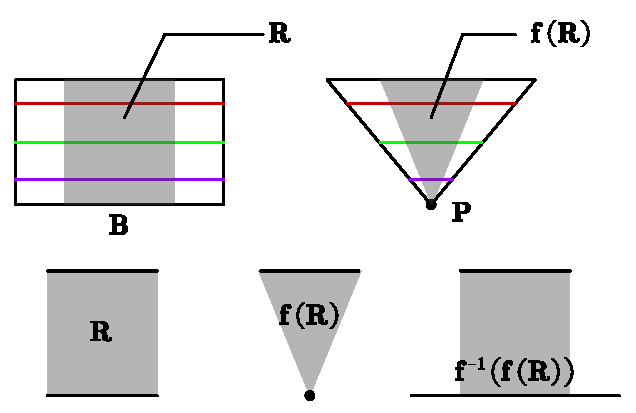
\includegraphics[width=10cm]{./figures/Topo7_7.pdf}
\caption{$A$,$R$,$B$,$A/\sim$,$f(R)$和$f^{-1}(f(R))$的示意图.图中阴影部分表示$R$或$f(R)$.可见$f^{-1}(f(R))$和$R$相比,底边两端突出了,不再是$X$的开集,因此$f(R)$不是$X/\sim$的开集.} \label{Topo7_fig7}
\end{figure}

\end{example}

由\autoref{Topo7_ex2}可见,$X$和$X/\sim$的开集不一定都会一一对应.

